
\newcommand{\imagw}[3]{
  \begin{figure}[!hbt]
    \centering
    \includegraphics[width=#1]{#2}
    \caption{#3}
    \label{fig:#2}
  \end{figure}
}

\newcommand{\imag}[2]{\imagw{16cm}{#1}{#2}}

\chapter{Setup for spatio-angular illumination}
\begin{summary}
  We build something
\end{summary}

\nomenclature{MEMI}{Micro-mirror enhanced micro-imaging. EU FP7
  project reference 215597.}


\begin{figure}[!hbt]
  \centering
  \def\svgscale{1.5}
  \input{memi-simple.eps_tex}
  \caption{Simplified schematic of the MEMI system. Light coming from
    the source is homogenized in an integrating tunnel. The light then
    traverses two spatial light modulators. The first of which (MMA)
    is imaged into the back focal plane of the objective and the
    second (LCoS) into the sample.}
  \label{fig:memi-simple}
\end{figure}



\begin{figure}
   \centering
   \def\svgscale{2}
   \input{memi-sketch.eps_tex}
   \caption{Schematic of the lenses in the MEMI system and their focal
     lengths. The focal length $f_\textrm{TL}$ of the tubelens can be
     varied. This allows to scale the second intermediate image
     $r''_\textrm{MMA}$ of the micro mirror array to fit the back
     focal plane of different objectives. Dimensions in mm.}
   \label{fig:memi-sketch}
 \end{figure}


\figref{fig:setup-gimp} shows a schematic of the light path in
the combined angular and spatial control system. The distance between
either source or MMA and the lens L1 is equal to the focal distance ofo
L1. Therefore if all mirrors of the MMA are flat, an image of the
source is formed in the plane of the aperture B1. The size of the
aperture is chosen to transmit just this image. When mirrors of the
MMA are tilted, they will slightly deflect the light, so that it no
longer passes through the aperture.  In the schematic the left half of
the MMA mirrors are tilted. Therefore the right part of the back focal
plane of the objective L5 is not illuminated and the light pattern
that excites the fluorophores in the sample is only half of the
conventional "hourglass" double cone.

The lenses L2 and L3 relay the image of the source from B1 into the
LCoS plane.  The incoming light is linearly polarized and its electric
field vibrates in the plane of the paper. Depending its state (on or
off) the LCoS pixel can rotate the polarization of the returning
light, so that it is reflected towards the objective L5 by the
polarizing beam splitter PBS.


In the front focal plane of the objective L5 an image of the pattern
on the LCoS is formed. Excited fluorophores emit fluorescence photons
of which a certain solid angle is collected by the objective L5
(depicted as green ray bundle). The dichroic beam splitter D1 reflects
these photons down. The tube lens L4 forms an image of the fluorescent
object in the camera plane.


\imag{setup-gimp}{Schematic of the light path through our
  microscope. M1 and M2 are mirrors.  L1, L2, L3, L4 and L5 are
  lenses. B1 is an adjustable circular aperture. PBS is a polarizing
  beam splitter. D1 is a dichroitic beam splitter.}


\imag{setup-photo-blueprint}{The widefield epi-fluorescent microscope
  with attached illumination head. The positions of the two spatial
  light modulators (Micro mirror array (MMA) and liquid crystal on
  silicon display (LCoS)) are indicated.}

\imag{mma}{{\bf left:} Scanning electron microscope image of the
  micro-mirror array (MMA).  The pixel pitch of the device is
  \unit[0.016]{mm}. The hinges for the tilt movement and the
  electrodes are clearly visible. {\bf middle:} Optical reflective
  microscope image of the MMA. {\bf right:} exaggerated rendering of
  how a 8x8 checker board pattern would be displayed on the device.}

\imagw{8cm}{optimization}{bnla lba}

\begin{figure}[!hbt]
  \centering
  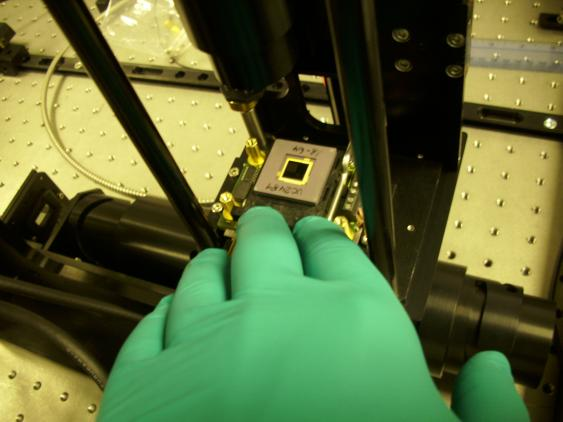
\includegraphics[width=7cm]{mma-plain}
  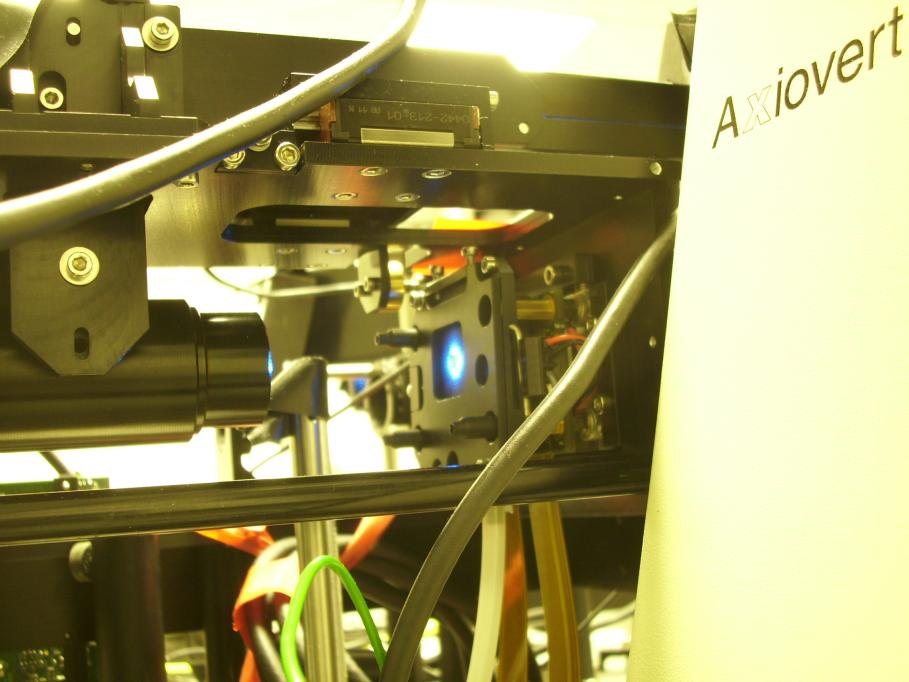
\includegraphics[width=7cm]{mma-ill}
  \caption{{\bf left:} Micro mirror array chip during installation of
    the optics. {\bf right:} Illuminated micro mirror array in the
    aligned system.}
  \label{fig:mma-closeup}
\end{figure}

\begin{figure}[!hbt]
  \centering
  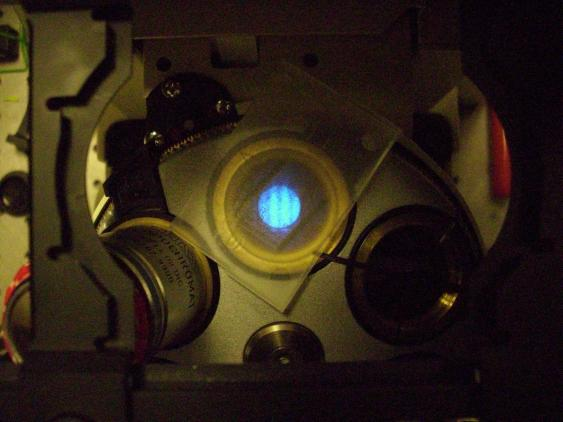
\includegraphics[width=7cm]{bfp1}
  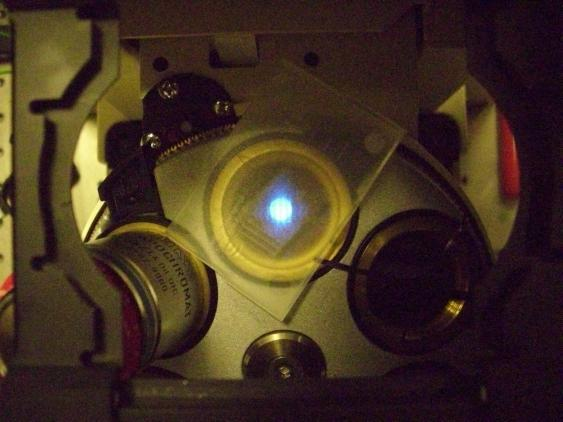
\includegraphics[width=7cm]{bfp2}
  \caption{Images of the micro mirror array in the back focal plane
    with different settings of the variable tubelens.}
  \label{fig:mma-closeup}
\end{figure}

\imagw{5cm}{lcos}{lcos}

